\documentclass{llncs}
\usepackage[utf8]{inputenc}
\usepackage[T1]{fontenc}
\usepackage{graphicx}

\graphicspath{{resources/}}
\newcommand\tab[1][0.5cm]{\hspace*{#1}}

\begin{document}

\title{ConfiguraFácil}
\author{Alexandre Pinho, Joel Gama, Tiago Pinheiro}

\institute{
University of Minho, Department of  Informatics, 4710-057 Braga, Portugal, \\
\email{a82441@alunos.uminho.pt},\email{a82202@alunos.uminho.pt},\email{a82491@alunos.uminho.pt}
}

\maketitle

\clearpage

\section{Introdução}

Este projeto surge no âmbito da UC de Desenvolvimento de Sistemas de Software, que faz parte do Mestrado Integrado em Engenharia Informática, da Universidade do Minho.

\tab Foi-nos proposto desenvolver um sistema que tem dois principais usos: a encomenda de um carro segundo uma configuração escolhida pelo cliente; e a utilização do software no chão da fábrica, que inclúi o registo da chegada de componentes e a gestão da fila de espera da produção dos carros. 

\tab As seguintes secções descrevem o processo de desenvolvimento do projeto seguido pelo grupo, as escolhas de design da arquitetura feitas pelo grupo, e o resultado final obtido. Por fim, é feita uma análise crítica ao trabalho desenvolvido.

\clearpage
\section{Processo de desenvolvimento}

\tab O processo de desenvolvimento do projeto baseou-se no que foi lecionado nas aulas: é dada uma atenção especial ao planeamento organizado da estrutura da aplicação tendo em conta os requerimentos funcionais identificados com o cliente.

\subsection{Modelação do domínio}

O primeiro passo no processo de desenvolvimento consiste na modelação do domínio do problema. Representam-se gráficamente as entidades do problema e os relacionamentos entre si. Esta fase é a melhor ocasião para esclarecer quaisquer dúvidas ou inconsistências com o cliente. No fim, já é possível começar a identificar os principais conceitos e funcionalidades da aplicação, a ser especificados posteriormente.

\begin{figure}
\begin{center}
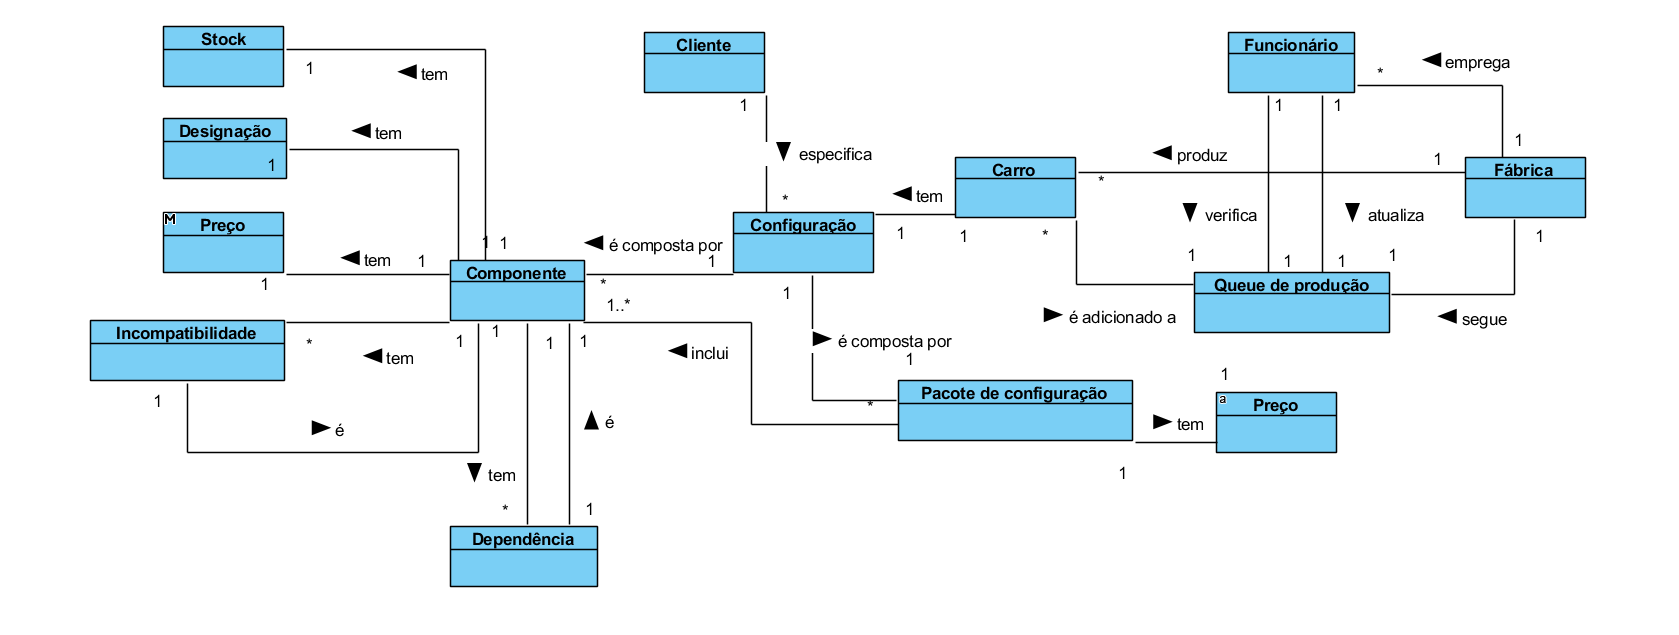
\includegraphics[scale=0.25]{modelo_de_dominio.png} 
\end{center}
\caption{\label{fig:modelo_dominio}Modelo de domínio}
\end{figure} 


\tab Como podemos visualizar na figura \ref{fig:modelo_dominio}, o grupo identificou, para além das características básicas de um componente e entidades auxiliares, várias entidades principais: o componente, o pacote de configuração, a configuração, o cliente, o carro, e a queue de producao. 

\subsection{Modelação dos requesitos funcionais}

Com a modelação do domínio do problema feita, é necessário identificar os requesitos funcionais da aplicação, ou seja, os diferentes casos de uso (Use Cases) da aplicação. Esta modelação é importante por várias razões: para além de identificar o que a aplicação faz em concreto e facilitar o teste da aplicação, também serve para esclarecer, tanto para o programador como para o cliente, o que a aplicação não faz.

\begin{figure}
\begin{center}
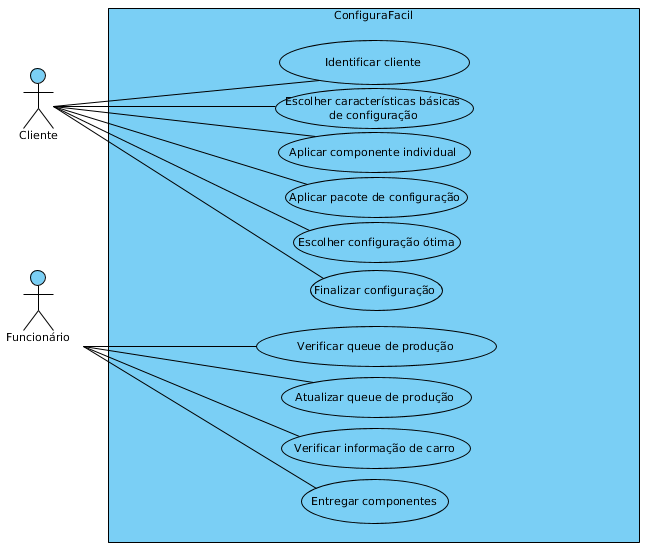
\includegraphics[scale=0.40]{diagrama_use_cases.png} 
\end{center}
\caption{\label{fig:diagrama_use_cases}Diagrama de Use Cases}
\end{figure} 

\tab Na aplicação a desenvolver neste projeto foram identificados dois atores (cliente e funcionário) e dez Use Cases. O diagrama de Use Cases da figura \ref{fig:diagrama_use_cases} representa gráficamente esta informação.

\subsection{Especificação dos Use Cases}

\begin{figure}
\begin{center}
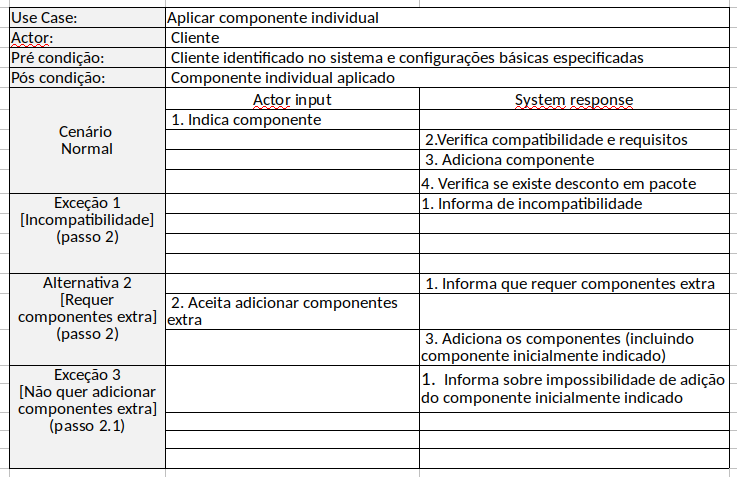
\includegraphics[scale=0.40]{aplicar_componente_tabular.png} 
\end{center}
\caption{\label{fig:notacao_tabular}Especificação do Use Case "Aplicar componente individual" em notação tabular }
\end{figure} 

Depois de identificados os Use Cases é feita a sua especificação, representando em notação tabular a interação entre o ator e o sistema, como por exemplo na figura \ref{fig:notacao_tabular}.

\subsection{Conceção da interface}

De forma a consultar com o cliente e ter o seu feedback, foi desenvolvido na fase inicial do projeto um protótipo de baixa fidelidade do aspeto da interface, e foi desenhado um diagrama de máquinas de estado a descrever o comportamento da interface. Embora o desenho da interface tenha mudado ao longo do desenvolvimento da aplicação, as ideias básicas são as mesmas, não sendo o produto final fundamentalmente diferente.

\subsection{Modelação comportamental}

A partir da especificação de um Use Case, através da sua transformação num diagrama de sequência de sistema (DSS) e da adição de cada vez mais detalhes de implementação, é possível ter um (ou vários) diagrama de sequência que modelam o comportamento do sistema. Os diagramas de sequência, se suficientemente detalhados, podem até servir para gerar automaticamente grandes parte do código da aplicação. O diagrama de classes permite também modelar o comportamento da aplicação, pois detalha as várias classes com métodos e atributos, e a sua relação com as outras classses do código.

\tab O processo seguido pelo grupo consiste em desenvolver em paralelo os diagramas de sequência e de classes para cada Use Case, e desenvolver cada conjunto de diagramas de um Use Case em paralelo com o resto dos Use Cases, comunicando entre os membros do grupo para manter o desenho da arquitetura de classes consistente.

\subsubsection{Persistência.} % nova linha se possível

Parte do processo de modelação comportamental consiste em transformar os diagramas feitos da perspetiva de que toda a informação da aplicação será guardada em memória central, em diagramas onde se considera a necessidade desta informação poder ser utilizada em mais que uma execução da aplicação. O método utilizado garantiu que esta mudança fosse feita com poucas dificuldades pois a persistência foi abstraida e modularizada em classes DAO (Data Access Object), que são fáceis de integrar pois implementam métodos similares às classes utilizadas anteriormente.

\begin{figure}
\begin{center}
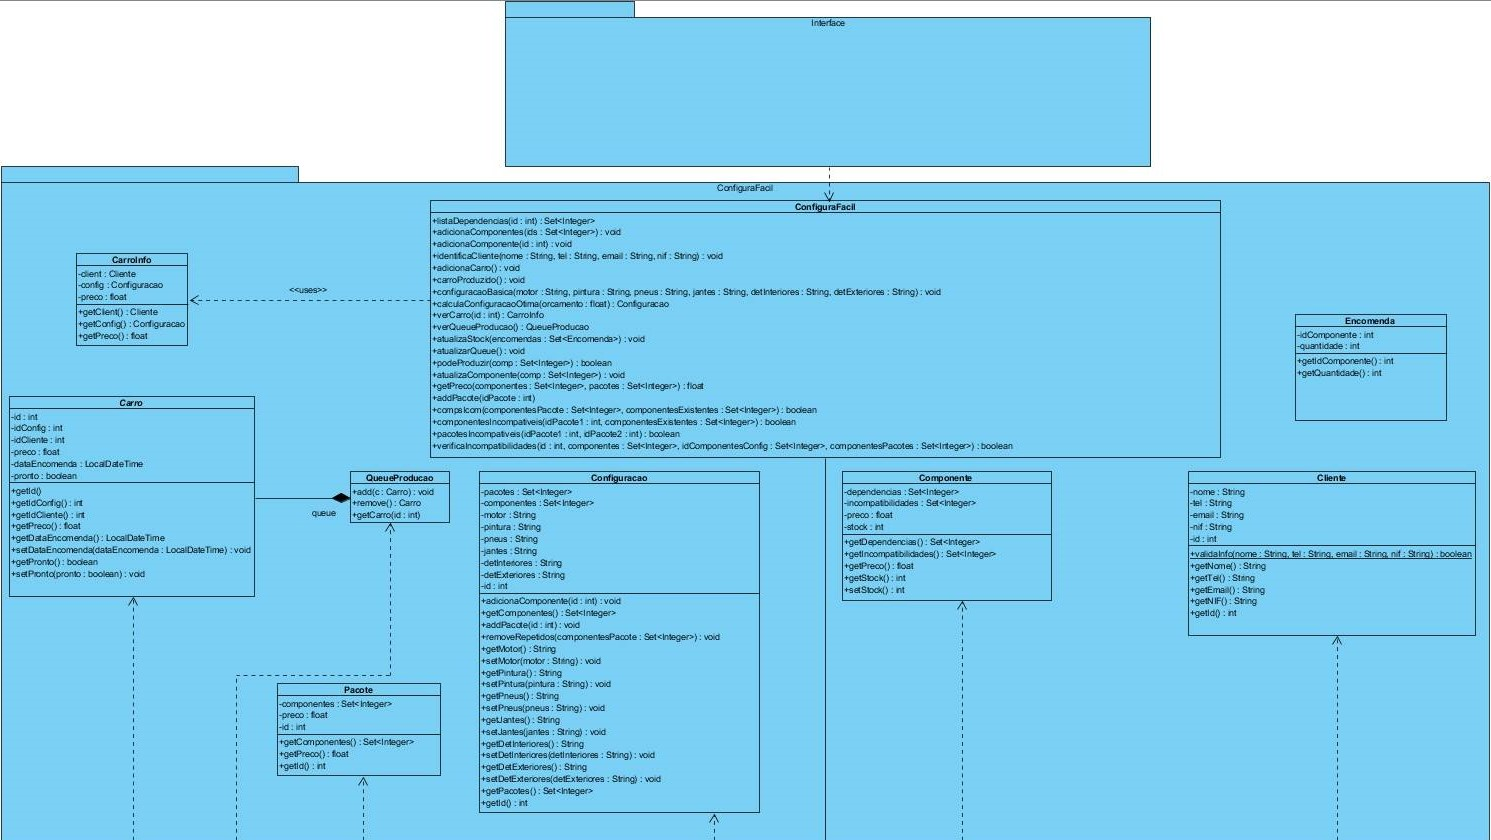
\includegraphics[scale=0.33]{diagrama_classes_global1.png}
\end{center}
\caption{\label{fig:diagrama_classes_global1}Diagrama de classes global1}
\end{figure}

\begin{figure}
\begin{center}
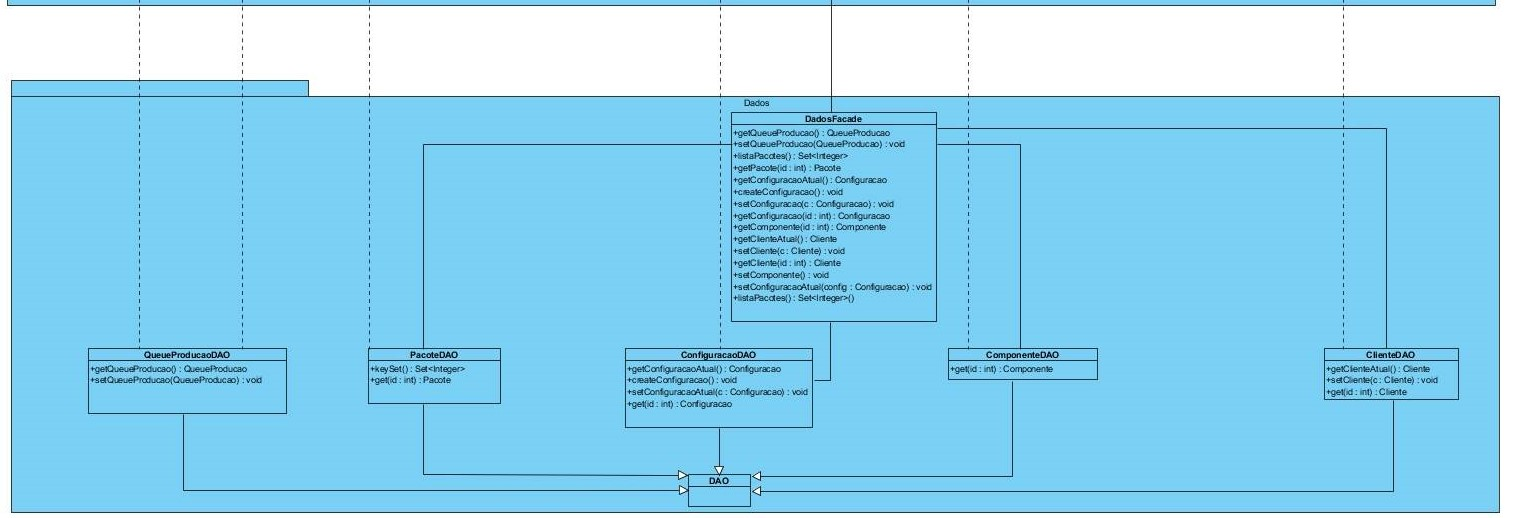
\includegraphics[scale=0.33]{diagrama_classes_global2.png}
\end{center}
\caption{\label{fig:diagrama_classes_global2}Diagrama de classes global2}
\end{figure}

\tab No fim da modelação do comportamento de todos os Use Cases individualmente, é feito o diagrama de classes global, que junta a informação dos outros diagramas de classes, e adiciona packages e as suas classes Facade (se ainda não existirem), como mostra nas figuras \ref{fig:diagrama_classes_global1} e \ref{fig:diagrama_classes_global2}.

\clearpage
\section{Conceção da solução} % título de secção melhor?

O código desenvolvido está estruturado à volta de uma arquitetura de classes organizadas por camadas, sendo as classes de cada camada postas num package dedicado. Assim, a aplicação tem três camadas: a camada de interface, a camada de negócio, e a camada de dados.

\tab A camada da interface é responsável pela interação do utilizador da aplicação com o sistema. Para isto, a camada contém classes que servem para abrir janelas que recebem input do utilizador e prestam a este a informação pretendida. Para o desenvolvimento desta camada foi utilizada principalmente a framework SWING.

\tab A camada de negócio é responsável pela implementação da lógica de negócio da aplicação. Por exemplo, é responsável por adicionar um componente à configuração atual quando assim é pedido pelo utilizador. A camada de negócio fornece uma interface face à camada de interface, e utiliza métodos fornecidos pela camada de dados.

\tab A camada de dados é responsável por implementar a persistência dos dados da aplicação. Através da utilização de uma base de dados relacional (MySQL), é guardada a informação dos componentes e pacotes existentes, bem como o cliente e configuração atuais e os carros na linha de produção.

\subsection{Camada de interface}

Para o desenvolvimento da interface foi seguida a arquitetura MVC (Model-view-controller). Com esta arquitetura existe uma separação entre a representação da informação e a interação do usuário com ela.

\tab Esta arquitetura divide uma aplicação em três partes interconectadas, modelo, vista e controladores. Desta forma existe separação das representações de informação internas dos modos como a informação é apresentada e aceite pelo utilizador. O padrão de projetos MVC separa os componentes maiores, possibilitando a reutilização de código e o desenvolvimento paralelo de forma eficiente. 

\tab Seguindo esta arquitetura a interface desenvolvida iniciasse com o "Menu Inicial" onde é possível decidir se se quer iniciar a aplicação no modo "Vendedor", modo que permite configurar um carro, ou no modo "Fabricante", modo a usar no chão da fábrica.
Quando o modo "Vendedor" é iniciado é pedido para que o cliente se identifique, introduzindo os seus dados. Quando a identificação for concluída o cliente pode proceder à escolha das características básicas de configuração. Depois deste passo é aberta uma janela com a configuração atual do cliente e três opções de configuração avançada, "Adicionar Pacote", "Adicionar Componente Individual" e "Solução Ótima". Na opção "Adicionar Pacote" pode ser adicionado um ou mais pacotes dos quatro pacotes definidos no sistema, desde que não existam incompatibilidades. Quando um pacote é selecionado na janela são mostrados os componentes e preço do pacote. Já na opção "Adicionar Componente Individual" é possível adicionar um componente individual. Primeiro é necessário selecionar o id do componente a adicionar e depois de verificar as dependências e incompatibilidades (mostradas na janela) pode ser adicionado o componente e todos os componentes de que este é dependente. A opção "Solução Ótima" mostra, mediante um orçamento fornecido, a melhor solução disponível no sistema. Por fim, clicando em "Próximo" na janela de opções avançadas procede-se à finalização da encomenda. Nesta última janela do modo "vendedor" é possível observar a configuração final do carro e o preço.

\tab O modo "Fabricante" tem quatro opções disponíveis. "Verificar Queue de Produção", "Atualizar Produção", "Verificar Carro" e "Entregar Componentes". Na opção de "Verificar Queue de Produção" é possível ver todos os carros que estão em espera para serem produzidos, bem como a informação de que se podem ou não ser produzidos. "Atualizar Produção" remove o primeiro carro da queue de produção se este tiver stock disponível para produção. A opção "Verificar Carro" permite ver as informações de um carro dado o seu id. Por fim, "Entregar Componentes" permite que seja registada a chegada de stock, adicionando os componentes um a um numa lista, dado o seu id e a quantidade.

\subsection{Camada de negócio}

A camada de negócio contém a classe ConfiguraFacil, sendo esta a principal classe desta camada. A ConfiguraFacil possui todos os métodos que permitem responder ás várias funcionalidades da aplicação. Esta classe é o elo de ligação entre a interface e a camada de dados. Para conseguir efetuar a ligação à camada de dados ela possui uma variável privada, \textit{dados} da classe \textit{DadosFacade}, sendo inicializada através do construtor parametrizado.

\tab Para além da ConfiguraFacil, a camada possui as classes Carro, Cliente, Componente, Configuracao e Pacote que representam os objetos usados aplicação. Todas estas classes possuiem um identificador, \textit{id}, que é utilizado nas restantes classes. A escolha entre a utilização de um identificador ao invés de um objeto foi feita a pensar na base de dados, para ter custos de memória reduzidos. Desta forma, em vez de carregar para memória um objeto e ainda os objetos associados a que este faz referencia apenas é necessário carregar o objeto em questão e os identificadores dos outros objetos referenciados por este. 

\tab A classe CarroInfo é utilizada para retornar a informação de um carro que se encontra na queue, assim como da informação sobre o utilizador que o possuí e ainda da sua configuração.

\tab A classe Encomenda é usada para que o utilizador \textit{funcionário} adicione os componentes indiduais ao stock da fábrica.

\tab Por fim, esta camada utiliza ainda a classe QueueProducao. Esta classe contém os métodos que permitem adicionar e remover elementos da queue, e ainda consultar os elementos da mesma.

\subsection{Camada de dados}

\begin{figure}
\begin{center}
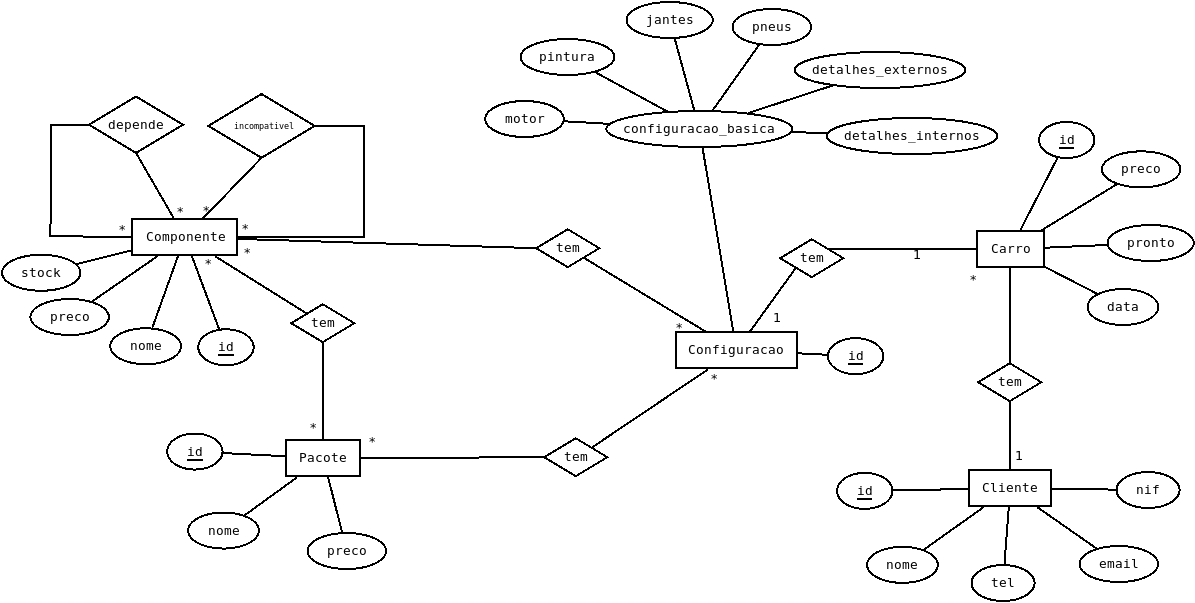
\includegraphics[scale=0.33]{esquema_conceptual.png}
\end{center}
\caption{\label{fig:esquema_conceptual}Esquema conceptual da base de dados}
\end{figure}

Como motor de base de dados, foi utilizado o MySQL pois tem um modelo relacional e devido à familiarididade com o sistema dos elementos do grupo.

\tab Como podemos verificar na figura \ref{fig:esquema_conceptual}, o esquema conceptual da base de dados, as classes escolhidas para representar a informação necessária foram as classes Carro, Cliente, Componente, Configuração e Pacote. Combinado com os restantes elementos (atributos e relacionamentos) do esquema, dá origem a um esquema físico com uma tabela para cada classe escolhida, e uma tabela para cada relacionamento N para N.

\tab A arquitetura de classes utiliza o padrão Facade para simplificar o acesso pela camada de negócio. A classe DadosFacade é responsável por iniciar a conexão à base de dados, de tratar da definição de transações, ao capturar qualquer exceção e nesse caso fazer rollback das mudanças.

\tab Existe uma classe DAO para cada classe escolhida para o esquema da base de dados, com a exceção da classe Carro. Isto deve-se ao facto dos carros estarem associados fortemente com a queue de produção, pelo que existe a classe QueueProducaoDAO para tratar dos carros nela presentes como uma estrutura apenas.

\tab Todas as classes de acesso de dados são subclasses da classe DAO. Esta classe implementa todo o comportamento em comum entre as suas subclasses, o que neste momento é apenas guardar uma referência ao objeto de conexão à base de dados, mas no futuro é possível acrescentar a este comportamento de necessário.

Assim, a camada de dados implementa as operações necessárias para o correto funcionamento da aplicação: o acesso e alteração da configuração (componentes individuais e pacotes), e o acesso e alteração da queue de produção.

\clearpage
\section{Conclusão}

Na realização deste trabalho foi utilizado um processo baseado no planeamento estruturado e organizado da arquitetura de modo a cumprir requisitos funcionais concretos. Seguindo este processo o resultado a que chegamos permite a encomenda de um carro segundo uma configuração escolhida pelo cliente; e a utilização do software no chão da fábrica, que inclúi o registo da chegada de componentes e a gestão da fila de espera da produção dos carros. 

\tab Em alguns aspetos poderia haver melhorias no trabalho realizado, nomeadamente a implementação de métodos mais específicos na camada de dados, desta forma não seria necessário carregar toda a informação dos componentes quando apenas se precisa de um atributo no momento. Outra melhoria seria, a partir de um processo iterativo, testar sistematicamente o programa (unit testing).

\end{document}
